\section{Rao/Sutton-Inspired Parametric Bell-Nozzle Geometry Formulation}
\label{sec:geometry}
% =========================================================

\subsection{Analytical contour definition}

\subsubsection{Independent geometric design parameters}

The nozzle geometry is defined by a reduced set of parameters:
\begin{itemize}
    \item throat radius, $r_t$;
    \item chamber radius, $r_c$;
    \item expansion ratio, $\varepsilon$;
    \item subsonic converging angle, $\theta_{sub}$;
    \item initial supersonic angle, $\theta_{in}$;
    \item reference conical half-angle, $\alpha$;
    \item bell length fraction, $K_b$, defined as a percentage of the reference conical length.
\end{itemize}

The geometric model follows classical bell-nozzle proportions described by Sutton and Biblarz, with circular throat arcs and a quadratic diverging section. It is a Rao/Sutton-inspired parametric contour, not a thrust-optimized Rao TOP contour obtained from a method-of-characteristics solution. The contour is axisymmetric, so the two-dimensional function $r(x)$ fully defines the three-dimensional surface by revolution around the nozzle axis.

\begin{figure}[H]
    \centering
    \IfFileExists{Images/RPE.png}{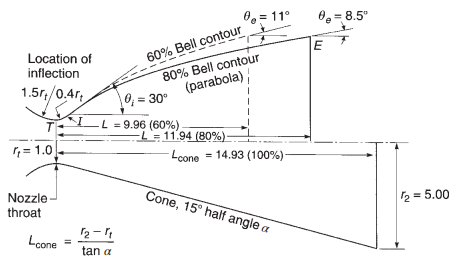
\includegraphics[width=0.82\linewidth]{Images/RPE.png}}{\IfFileExists{Images/RPE (1).png}{\includegraphics[width=0.82\linewidth]{Images/RPE (1).png}}{\fbox{\parbox{0.82\linewidth}{\centering Missing figure file: \texttt{RPE.png} or \texttt{RPE (1).png}}}}}
    \caption{Reference bell-nozzle proportions from the Sutton/Biblarz formulation.}
    \label{fig:RPE_geometry}
\end{figure}

\subsubsection{Global piecewise contour architecture}

The contour is constructed from four segments:
\begin{enumerate}
    \item initial straight converging line;
    \item subsonic circular arc upstream of the throat;
    \item supersonic circular arc immediately downstream of the throat;
    \item parabolic supersonic contour up to the exit plane.
\end{enumerate}

The coordinate origin is initially placed at the throat, with the nozzle axis along $x$ and the local radius along $r$. The throat point is therefore
\begin{equation}
(x_t,r_t)=(0,r_t).
\end{equation}

The full profile is later translated horizontally so that the exported and displayed geometry starts at $x=0$.

\subsubsection{Upstream throat-radius circular arc}

The subsonic circular arc uses a radius
\begin{equation}
R_{sub}=1.5r_t.
\end{equation}

Its center is placed on the radial axis at
\begin{equation}
C_{sub}=(0,2.5r_t).
\end{equation}

The circular equation is
\begin{equation}
x^2+(r-2.5r_t)^2=(1.5r_t)^2.
\end{equation}

The lower branch of the circle defines the desired arc:
\begin{equation}
r(x)=2.5r_t-\sqrt{(1.5r_t)^2-x^2},
\qquad x\in[x_r,0].
\label{eq:sub_arc}
\end{equation}

The connection point between the initial straight line and the subsonic arc is
\begin{align}
x_r &= -1.5r_t\sin(\theta_{sub}),
\label{eq:xr}\\
r_r &= 2.5r_t-1.5r_t\cos(\theta_{sub}).
\label{eq:yr}
\end{align}

\begin{figure}[H]
\centering
\begin{tikzpicture}[scale=1.75, line cap=round, line join=round]

% ---------------------------------------------------------
% Key points
% ---------------------------------------------------------
\coordinate (O) at (0,0);           % x=0 reference on x-axis
\coordinate (T) at (0,1.10);        % throat point
\coordinate (C) at (0,3.35);        % center of subsonic circle
\coordinate (Q) at (-1.299,1.85);   % connection point, on circle of radius 1.5

% ---------------------------------------------------------
% Axes
% ---------------------------------------------------------
\draw[black,
      dash pattern=on 8pt off 2pt on 1pt off 2pt,
      -latex] (-3.40,0) -- (1.80,0);    % x-axis
\draw[black,-latex] (0,-0.05) -- (0,4.35);      % vertical reference axis

% ---------------------------------------------------------
% Dashed construction lines
% ---------------------------------------------------------
\draw[densely dashed, gray] (Q) -- (Q |- O);      % vertical from Q to x-axis
\draw[densely dashed, gray] (Q) -- (0,1.85);      % horizontal from Q to y-axis
\draw[densely dashed, gray] (T) -- (O);           % vertical from throat to x-axis

% ---------------------------------------------------------
% Initial straight converging line
% ---------------------------------------------------------
\draw[black, line width=0.9pt] ($(Q)+(-1.75,1.75)$) -- (Q);

\draw[black, line width=0.9pt, -latex] (-3.5,0.75) -- (-2.25,0.75);

\draw[black, line width=0.9pt, -latex] (-3.5,1.05) -- (-2.25,1.05);

\draw[black, line width=0.9pt, -latex] (-3.5,0.9) -- (-2,0.9);

\node at (-2.675,1.2) {$\dot{m}_{\text{prop}}$};
% ---------------------------------------------------------
% Subsonic arc (lower branch of circle)
% Circle center C=(0,2.60), radius=1.5
% From Q to T
% ---------------------------------------------------------
\draw[black, line width=0.9pt]
    (Q) arc[start angle=210, end angle=270, radius=1.5];

% ---------------------------------------------------------
% Red auxiliary geometry
% ---------------------------------------------------------

% Horizontal reference through Q
\draw[red!70!black,dashed , line width=0.7pt] (-2.25,1.85) -- (Q);

% Radius from center to Q
\draw[red!70!black, dashed, line width=0.8pt] (C) -- (Q);

% Vertical reference from center downward
\draw[red!70!black, dashed, line width=0.8pt] (C) -- (0,1.10);

% ---------------------------------------------------------
% Point marker at Q
% ---------------------------------------------------------
\filldraw[white] (Q) circle (1.5pt);
\draw (Q) circle (2 pt);

% ---------------------------------------------------------
% Angle theta_sub at Q (between left horizontal and tangent line)
% ---------------------------------------------------------
\draw[black]
    ($(Q)+(-0.34,0)$) arc[start angle=180, end angle=135, radius=0.34];
\node[anchor=east] at ($(Q)+(-0.42,0.2)$) {$\theta_{\text{sub}}$};

% ---------------------------------------------------------
% Angle theta_sub at C (between downward vertical and radius CQ)
% ---------------------------------------------------------
\draw[red!70!black]
    ($(C)+(0,-0.42)$) arc[start angle=-90, end angle=-130, radius=0.42];
\node[anchor=west] at ($(C)+(-0.5,-0.74)$) { $\theta_{\text{sub}}$};

% ---------------------------------------------------------
% Radius label
% ---------------------------------------------------------
\node[anchor=west] at (-1.25,2.7) {$1.5r_t$};
\coordinate (F) at ($(Q)+(-1.75,1.75)$);

\draw[black, line width=0.9pt] (F) -- (Q);

\draw[densely dashed, gray] (F) -- (0,3.6);
\draw[densely dashed, gray] (F) -- (-1.299-1.75,0);


\node[anchor=west] at (0,3.6) {$r_{in}$};
% ---------------------------------------------------------
% Labels
% ---------------------------------------------------------
\node[anchor=north] at (-1.299,0) {$x_r$};
\node[anchor=north] at (0,0) { $0$};
\node[anchor=west]  at (0,1.85) {$y_r$};
\node[anchor=west]  at (0,4.35) { $y_r$};
\node[anchor=west]  at (T) { $r_t$};
\node[anchor=north] at (1.75,0) { $x$};
\node[below left=2pt] at (Q) {$Q$};
% ---------------------------------------------------------
% Q coordinate box
% ---------------------------------------------------------
\draw[black] (1.05,1.72) rectangle (2.80,2.25);
\node at (1.925,1.985) {$Q=(x_r,y_r)$};

\end{tikzpicture}
\caption{Subsonic geometric relations and definition of the converging arc.}
\label{fig:subsonic_geometry_tikz}
\end{figure}

\subsubsection{Linear converging-section approximation}

The initial converging section is approximated as a straight line tangent to the subsonic arc at $(x_r,r_r)$. Its slope is set by the angle $\theta_{sub}$:
\begin{equation}
m_{sub}=-\tan(\theta_{sub}).
\end{equation}

The line equation is
\begin{equation}
r(x)=m_{sub}x+b_{sub},
\end{equation}
where
\begin{equation}
b_{sub}=r_r-m_{sub}x_r.
\end{equation}

Substituting Eqs.~\eqref{eq:xr} and~\eqref{eq:yr}, the line can also be written as
\begin{equation}
r(x)=-\tan(\theta_{sub})x
+r_t\left[2.5-1.5\cos(\theta_{sub})-1.5\sin(\theta_{sub})\tan(\theta_{sub})\right].
\label{eq:line_expanded}
\end{equation}

The first axial coordinate $x_f$ is obtained from the chamber radius condition,
\begin{equation}
r(x_f)=r_c,
\end{equation}
which gives
\begin{equation}
x_f=\frac{r_c-b_{sub}}{m_{sub}} .
\label{eq:xf}
\end{equation}

The contraction ratio is then
\begin{equation}
CR=\frac{A_c}{A_t}=\frac{r_c^2}{r_t^2}.
\label{eq:contraction_ratio}
\end{equation}

\subsubsection{Downstream throat-radius circular arc}

Immediately downstream of the throat, the supersonic arc uses radius
\begin{equation}
R_{sup}=0.4r_t.
\end{equation}

Its center is placed at
\begin{equation}
C_{sup}=(0,1.4r_t).
\end{equation}

The circular equation is
\begin{equation}
x^2+(r-1.4r_t)^2=(0.4r_t)^2.
\end{equation}

The branch used for the nozzle profile is
\begin{equation}
r(x)=1.4r_t-\sqrt{(0.4r_t)^2-x^2},
\qquad x\in[0,x_P].
\label{eq:sup_arc}
\end{equation}

Equivalently, the arc can be parameterized by the angle $\theta$:
\begin{align}
x(\theta)&=0.4r_t\cos\theta,\\
r(\theta)&=1.4r_t-0.4r_t\sin\theta,
\end{align}
with
\begin{equation}
\theta\in\left[\frac{\pi}{2},\frac{\pi}{2}-\theta_{in}\right].
\end{equation}

The final point of the arc is the beginning of the parabolic contour:
\begin{align}
x_P &=0.4r_t\sin(\theta_{in}),
\label{eq:xP}\\
r_P &=1.4r_t-0.4r_t\cos(\theta_{in}).
\label{eq:yP}
\end{align}

\begin{figure}[H]
\centering
\begin{tikzpicture}[scale=1.75, line cap=round, line join=round]

% ---------------------------------------------------------
% Parameters
% ---------------------------------------------------------
\pgfmathsetmacro{\thetaInDeg}{35}
\pgfmathsetmacro{\Rsup}{0.80}      % schematic radius representing 0.4 rt
\pgfmathsetmacro{\Cy}{1.90}        % center of supersonic arc
\pgfmathsetmacro{\Ty}{\Cy-\Rsup}   % throat point y-coordinate

\pgfmathsetmacro{\Px}{\Rsup*sin(\thetaInDeg)}
\pgfmathsetmacro{\Py}{\Cy-\Rsup*cos(\thetaInDeg)}

\pgfmathsetmacro{\xE}{5.25}        % exit x-position (Lfinal)
\pgfmathsetmacro{\yE}{3.10}        % exit radius re

% Parabola coefficients:
% y(Px)=Py, y'(Px)=tan(theta_in), y(xE)=yE
\pgfmathsetmacro{\mP}{tan(\thetaInDeg)}
\pgfmathsetmacro{\den}{\xE-\Px}
\pgfmathsetmacro{\aPar}{(\yE-\Py-\mP*(\den))/(\den*\den)}
\pgfmathsetmacro{\bPar}{\mP-2*\aPar*\Px}
\pgfmathsetmacro{\cPar}{\Py-\aPar*\Px*\Px-\bPar*\Px}

\pgfmathsetmacro{\mE}{2*\aPar*\xE+\bPar}
\pgfmathsetmacro{\thetaOutDeg}{atan(\mE)}

% ---------------------------------------------------------
% Key points
% ---------------------------------------------------------
\coordinate (O) at (0,0);                    % x=0 reference
\coordinate (T) at (0,\Ty);                  % throat point
\coordinate (C) at (0,\Cy);                  % center of supersonic arc
\coordinate (P) at (\Px,\Py);                % transition point
\coordinate (E) at (\xE,\yE);                % nozzle exit point

% ---------------------------------------------------------
% Axes
% ---------------------------------------------------------
\draw[black,
      dash pattern=on 8pt off 2pt on 1pt off 2pt,
      -latex] (-0.25,0) -- (6.15,0);        % x-axis
\draw[black,-latex] (0,-0.05) -- (0,4.25);  % y-axis

% ---------------------------------------------------------
% Dashed construction lines
% ---------------------------------------------------------
\draw[densely dashed, gray] (P) -- (P |- O);     % vertical from P to x-axis
\draw[densely dashed, gray] (P) -- (0,\Py);      % horizontal from P to y-axis
\draw[densely dashed, gray] (E) -- (E |- O);     % vertical from exit to x-axis
\draw[densely dashed, gray] (E) -- (0, \yE);     % vertical from exit to x-axis

% ---------------------------------------------------------
% Supersonic arc (circular)
% ---------------------------------------------------------
\draw[black, line width=0.9pt]
    (T) arc[start angle=-90, end angle={-90+\thetaInDeg}, radius=\Rsup];

% ---------------------------------------------------------
% Parabolic divergent contour
% ---------------------------------------------------------
\draw[black, line width=0.9pt]
    plot[domain=\Px:\xE, samples=250]
    (\x,{\aPar*\x*\x+\bPar*\x+\cPar});

% ---------------------------------------------------------
% Red auxiliary geometry
% ---------------------------------------------------------

% Vertical reference from center to throat
\draw[red!70!black, dashed, line width=0.8pt] (C) -- (T);

% Radius from center to P
\draw[red!70!black, dashed, line width=0.8pt] (C) -- (P);

% Horizontal reference through P
\draw[red!70!black, dashed, line width=0.7pt] (P) -- ++(0.85,0);

% Small tangent reference at P
\draw[red!70!black, line width=0.7pt]
    ($(P)+(-0.15,-0.10)$) -- ++(\thetaInDeg:1.15);

% Exit tangent reference
\draw[red!70!black, line width=0.7pt]
    (E) -- ++(0.90,0);
\draw[red!70!black, line width=0.7pt]
    (E) -- ++(\thetaOutDeg:0.90);

% ---------------------------------------------------------
% Point marker at P
% ---------------------------------------------------------
\filldraw[white] (P) circle (1.5pt);
\draw (P) circle (2 pt);

% ---------------------------------------------------------
% Angle theta_in at P
% ---------------------------------------------------------
\draw[black]
    ($(P)+(0.34,0)$) arc[start angle=0, end angle=\thetaInDeg, radius=0.34];
\node[anchor=west] at ($(P)+(0.4,0.13)$) {$\theta_{\text{in}}$};

% ---------------------------------------------------------
% Angle theta_in at C
% ---------------------------------------------------------
\draw[red!70!black]
    ($(C)+(0,-0.42)$) arc[start angle=-90, end angle={-90+\thetaInDeg}, radius=0.42];
\node[anchor=west] at ($(C)+(0,-0.54)$) {$\theta_{\text{in}}$};

% ---------------------------------------------------------
% Angle theta_out at E
% ---------------------------------------------------------
\draw[red!70!black]
    ($(E)+(0.36,0)$) arc[start angle=0, end angle=\thetaOutDeg, radius=0.36];
\node[anchor=west] at ($(E)+(0.95,0.18)$) {$\theta_{\text{out}}$};


% ---------------------------------------------------------
% Radius label
% ---------------------------------------------------------
\node[anchor=west] at (0.15,1.65) {$0.4r_t$};

% ---------------------------------------------------------
% Labels
% ---------------------------------------------------------
\node[anchor=north] at (\Px,0) {$P_x$};
\node[anchor=north] at (0,0) {$0$};
\node[anchor=east]  at (0,\Py+0.1) {$P_y$};
\node[anchor=east] at ($(T)+(0,-0.1)$) {$r_t$};
\node[anchor=east]  at (0, \yE) {$r_e$};
\node[anchor=north] at (\xE,0) {$L_{\text{final}}$};
\node[anchor=west]  at (0,4.22) {$y$};
\node[anchor=north] at (6.10,0) {$x$};
\node[below right=1pt] at (P) {$P$};

% ---------------------------------------------------------
% P coordinate box
% ---------------------------------------------------------
\draw[black] (2.05,3.28) rectangle (3.80,3.81);
\node at (2.925,3.545) {$P=(P_x,P_y)$};

\draw[black, line width=0.9pt, -latex] (3,1.2) -- (4.5,1.2);

\draw[black, line width=0.9pt, -latex] (3,1.05) -- (4.75,1.05);

\draw[black, line width=0.9pt, -latex] (3,0.9) -- (4.5,0.9);

\node at (3.675,1.5) {$\dot{m}_{\text{prop}}$};

\end{tikzpicture}
\caption{Supersonic throat arc and transition into the parabolic diverging contour.}
\label{fig:supersonic_geometry_tikz}
\end{figure}

\subsubsection{Reference conical length and bell shortening factor}

The reference conical nozzle length is computed from the exit radius, throat radius and conical half-angle $\alpha$:
\begin{equation}
L_{cone}=\frac{r_e-r_t}{\tan\alpha}.
\label{eq:Lcone}
\end{equation}

The bell nozzle uses only a fraction $K_b$ of this length:
\begin{equation}
L_{parab}=K_b L_{cone}.
\label{eq:Lparab}
\end{equation}

The final axial coordinate of the parabolic section in the throat-centered coordinate system is
\begin{equation}
L=x_P+L_{parab}.
\label{eq:Lfinal}
\end{equation}

\subsubsection{Parabolic diverging-contour closure}

The parabolic contour is written as
\begin{equation}
r(x)=ax^2+bx+c,\qquad x\in[x_P,L].
\label{eq:parabola}
\end{equation}

A general parabola has three coefficients, so three independent conditions are imposed:
\begin{align}
r(x_P)&=r_P,
\label{eq:par_cond1}\\
r'(x_P)&=\tan(\theta_{in}),
\label{eq:par_cond2}\\
r(L)&=r_e.
\label{eq:par_cond3}
\end{align}

The first condition enforces positional continuity with the supersonic arc. The second condition enforces slope continuity and guarantees a smooth transition between the circular arc and the parabola. The third condition fixes the exit radius and therefore the desired expansion ratio.

The ideal case could also impose an exit angle condition,
\begin{equation}
r'(L)=\tan(\theta_{out}),
\end{equation}
but this would overdefine a simple parabola. Therefore, in the present formulation, $\theta_{out}$ is not prescribed; it is an output of the geometry.

The coefficient system is
\begin{equation}
\begin{bmatrix}
x_P^2 & x_P & 1\\
2x_P & 1 & 0\\
L^2 & L & 1
\end{bmatrix}
\begin{bmatrix}
a\\b\\c
\end{bmatrix}
=
\begin{bmatrix}
r_P\\ \tan(\theta_{in})\\ r_e
\end{bmatrix}.
\label{eq:parabola_matrix}
\end{equation}

Solving this linear system gives the parabolic coefficients that fully define the diverging section.

\subsubsection{Exit-plane wall angle}

The exit angle is obtained from the slope of the parabolic contour evaluated at the nozzle exit plane:
\begin{equation}
\theta_{out}=\arctan\left(2aL+b\right).
\label{eq:theta_out}
\end{equation}

This angle represents the local divergence of the flow at the nozzle exit and directly affects axial momentum efficiency. A large exit angle increases the radial velocity component and reduces useful axial thrust.

\subsubsection{Complete piecewise radius function}

Using the previous relations, the complete throat-centered nozzle contour can be written as
\begin{equation}
r(x)=
\begin{cases}
-\tan(\theta_{sub})x+b_{sub},
& x\in[x_f,x_r],\\[6pt]
2.5r_t-\sqrt{(1.5r_t)^2-x^2},
& x\in[x_r,0],\\[6pt]
1.4r_t-\sqrt{(0.4r_t)^2-x^2},
& x\in[0,x_P],\\[6pt]
ax^2+bx+c,
& x\in[x_P,L].
\end{cases}
\label{eq:piecewise_nozzle}
\end{equation}

This equation is one of the most important outputs of the geometric formulation because it gives a continuous mathematical representation of the entire nozzle contour.

% =========================================================
\subsubsection{Geometric station and angle summary}
% =========================================================

An illustrative nozzle geometry corresponding to $\varepsilon=5.0$ and $r_t=\SI{0.020}{m}$ is presented in Fig.~\ref{fig:nozzle_piecewise_tikz} to identify the stations and angles introduced in the previous sections.

\begin{figure}[H]
\centering
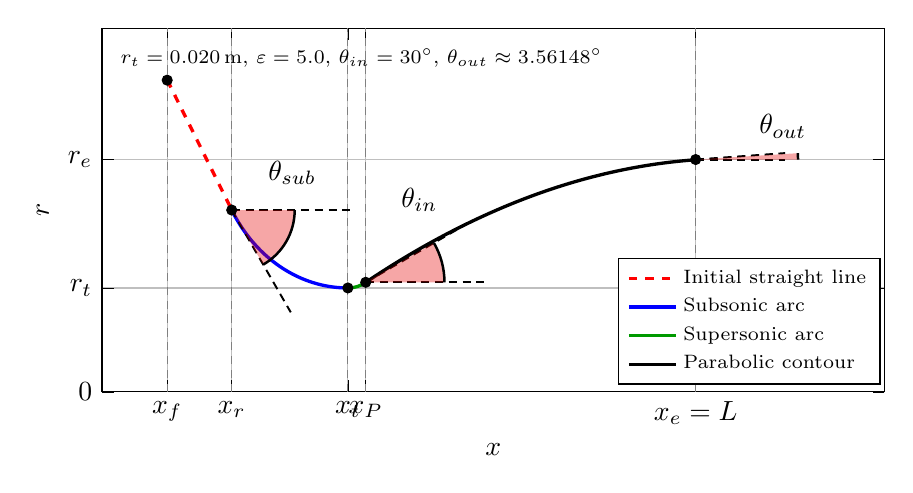
\begin{tikzpicture}
\begin{axis}[
    width=0.95\linewidth,
    height=6.2cm,
    grid=both,
    xlabel={$x$},
    ylabel={$r$},
    xmin=0, xmax=0.175,
    ymin=0, ymax=0.07,
    trig format=deg,
    scaled ticks=false,
    tick style={black},
    legend style={at={(0.995,0.02)},anchor=south east,fill=white,draw=black,line width=0.4pt,font=\scriptsize},
    legend cell align=left,
]

\pgfmathsetmacro{\rt}{0.020}
\pgfmathsetmacro{\eps}{5.0}
\pgfmathsetmacro{\re}{sqrt(\eps)*\rt}
\pgfmathsetmacro{\alphaDeg}{15}
\pgfmathsetmacro{\bell}{0.80}
\pgfmathsetmacro{\thetaSubDeg}{60}
\pgfmathsetmacro{\thetaInDeg}{30}
\pgfmathsetmacro{\Rch}{0.060}
\pgfmathsetmacro{\tx}{0.055}

\pgfmathsetmacro{\xr}{-1.5*\rt*sin(\thetaSubDeg)}
\pgfmathsetmacro{\yr}{2.5*\rt - 1.5*\rt*cos(\thetaSubDeg)}
\pgfmathsetmacro{\xR}{\tx+\xr}
\pgfmathsetmacro{\mLine}{-tan(\thetaSubDeg)}
\pgfmathsetmacro{\bLine}{\yr - \mLine*\xr}
\pgfmathsetmacro{\xf}{(\Rch - \bLine)/\mLine}
\pgfmathsetmacro{\xF}{\tx+\xf}

\pgfmathsetmacro{\rSup}{0.4*\rt}
\pgfmathsetmacro{\Px}{\rSup*sin(\thetaInDeg)}
\pgfmathsetmacro{\Py}{1.4*\rt - \rSup*cos(\thetaInDeg)}
\pgfmathsetmacro{\xP}{\tx+\Px}

\pgfmathsetmacro{\Lcone}{(\re-\rt)/tan(\alphaDeg)}
\pgfmathsetmacro{\L}{\Px + \bell*\Lcone}
\pgfmathsetmacro{\xE}{\tx+\L}
\pgfmathsetmacro{\mZero}{tan(\thetaInDeg)}
\pgfmathsetmacro{\den}{(\L-\Px)}
\pgfmathsetmacro{\aPar}{(\re - \Py - \mZero*(\den))/(\den*\den)}
\pgfmathsetmacro{\bPar}{\mZero - 2*\aPar*\Px}
\pgfmathsetmacro{\cPar}{\Py - \aPar*\Px*\Px - \bPar*\Px}
\pgfmathsetmacro{\thetaOutDeg}{atan(2*\aPar*\L + \bPar)}
\pgfmathsetmacro{\mOut}{tan(\thetaOutDeg)}

\pgfplotsset{
  xtick={\xF,\xR,\tx,\xP,\xE},
  xticklabels={$x_f$,$x_r$,$x_t$,$x_P$,$x_e=L$},
  ytick={0,\rt,\re},
  yticklabels={$0$,$r_t$,$r_e$},
}

\addplot[dashed, very thick, red, domain=\xF:\xR, samples=2] ({x},{\mLine*(x-\tx)+\bLine});
\addlegendentry{Initial straight line}

\addplot[very thick, blue, domain=\xR:\tx, samples=250] ({x},{2.5*\rt - sqrt((1.5*\rt)^2 - (x-\tx)^2)});
\addlegendentry{Subsonic arc}

\addplot[very thick, green!60!black, domain=\tx:\xP, samples=250] ({x},{1.4*\rt - sqrt((0.4*\rt)^2 - (x-\tx)^2)});
\addlegendentry{Supersonic arc}

\addplot[very thick, black, domain=\xP:\xE, samples=350] ({x},{\aPar*(x-\tx)^2 + \bPar*(x-\tx) + \cPar});
\addlegendentry{Parabolic contour}

\addplot[only marks, mark=*, mark size=1.8pt] coordinates {(\xF,\Rch) (\xR,\yr) (\tx,\rt) (\xP,\Py) (\xE,\re)};

\addplot[densely dashed, gray] coordinates {(\xF,0) (\xF,0.07)};
\addplot[densely dashed, gray] coordinates {(\xR,0) (\xR,0.07)};
\addplot[densely dashed, gray] coordinates {(\tx,0) (\tx,0.07)};
\addplot[densely dashed, gray] coordinates {(\xP,0) (\xP,0.07)};
\addplot[densely dashed, gray] coordinates {(\xE,0) (\xE,0.07)};

\path (axis cs:\xR,\yr) coordinate (Rpt);
\path (axis cs:\xP,\Py) coordinate (Ppt);
\path (axis cs:\xE,\re) coordinate (Ept);

\tikzset{angline/.style={densely dashed, black, line width=0.7pt}}

\def\Lsub{15mm}
\def\RadFillSub{8mm}
\def\RadArcSub{8mm}
\pgfmathsetmacro{\phiSub}{\thetaSubDeg}
\draw[angline] (Rpt) -- ++(\Lsub,0);
\draw[angline] (Rpt) -- ++(-\phiSub:\Lsub);
\fill[red!90!black, opacity=0.35] (Rpt) -- ++(\RadFillSub,0) arc[start angle=0, end angle=-\phiSub, radius=\RadFillSub] -- cycle;
\draw[black, line width=0.9pt] (Rpt) ++(\RadArcSub,0) arc[start angle=0, end angle=-\phiSub, radius=\RadArcSub];
\node[anchor=south west] at (axis cs:\xR+0.006,\yr+0.003) {$\theta_{sub}$};

\def\Lin{15mm}
\def\RadFillIn{10mm}
\def\RadArcIn{10mm}
\pgfmathsetmacro{\phiIn}{\thetaInDeg}
\draw[angline] (Ppt) -- ++(\Lin,0);
\draw[angline] (Ppt) -- ++(\phiIn:\Lin);
\fill[red!90!black, opacity=0.35] (Ppt) -- ++(\RadFillIn,0) arc[start angle=0, end angle=\phiIn, radius=\RadFillIn] -- cycle;
\draw[black, line width=0.9pt] (Ppt) ++(\RadArcIn,0) arc[start angle=0, end angle=\phiIn, radius=\RadArcIn];
\node[anchor=north] at (axis cs:\xP+0.012,\Py+0.02) {$\theta_{in}$};

\pgfmathsetmacro{\dxE}{0.020}
\draw[angline] (axis cs:\xE,\re) -- (axis cs:\xE+\dxE,\re);
\pgfmathsetmacro{\dyE}{\mOut*\dxE}
\draw[angline] (axis cs:\xE,\re) -- (axis cs:\xE+\dxE,\re+\dyE);
\pgfmathsetmacro{\phiOut}{\thetaOutDeg}
\def\RadFill{13mm}
\def\RadArc{13mm}
\path (Ept) ++(\RadFill,0) coordinate (FillStart);
\fill[red!90!black, opacity=0.35] (Ept) -- (FillStart) arc[start angle=0, end angle=\phiOut, radius=\RadFill] -- cycle;
\path (Ept) ++(\RadArc,0) coordinate (ArcStart);
\draw[black, line width=0.9pt] (ArcStart) arc[start angle=0, end angle=\phiOut, radius=\RadArc];
\node[anchor=center] at (rel axis cs:0.87,0.73) {$\theta_{out}$};

\node[anchor=north west] at (axis cs:0.002,0.068) {\scriptsize $r_t=\rt\,\mathrm{m}$, $\varepsilon=\eps$, $\theta_{in}=\thetaInDeg^\circ$, $\theta_{out}\approx\thetaOutDeg^\circ$};

\end{axis}
\end{tikzpicture}
\caption{Two-dimensional nozzle contour with region definitions, stations and angle notation.}
\label{fig:nozzle_piecewise_tikz}
\end{figure}

% =========================================================
\subsection{Numerical Coordinate Conditioning and Two-Dimensional Contour Output}
% =========================================================


\subsubsection{Axial coordinate translation}

The throat-centered coordinate system is convenient for mathematical construction, but it produces negative $x$ values in the subsonic converging section. For plotting, CAD export and easier interpretation, the profile is translated horizontally so that the first point of the nozzle starts at $x=0$.

The required translation is
\begin{equation}
\Delta x=-x_f.
\label{eq:translation_simple}
\end{equation}

Using the line geometry, this can also be written as
\begin{equation}
\Delta x=-x_r+\frac{r_c-y_r}{\tan(\theta_{sub})}.
\label{eq:translation}
\end{equation}

\begin{figure}[H]
\centering
\begin{tikzpicture}[scale=1.75, line cap=round, line join=round]

% ---------------------------------------------------------
% Key points
% ---------------------------------------------------------
\coordinate (O) at (0,0);            % x = 0 reference
\coordinate (T) at (0,1.10);         % throat point
\coordinate (C) at (0,3.35);         % center of subsonic circle
\coordinate (Q) at (-1.299,1.85);    % connection point
\coordinate (R) at (-3.05,3.75);     % inlet point: R=(xf,rchamber)

% Auxiliary points
\coordinate (Rf) at (R |- O);        % projection of R on x-axis
\coordinate (Rq) at (R |- Q);        % point at x=xf and y=yr
\coordinate (Qf) at (Q |- O);        % projection of Q on x-axis

% ---------------------------------------------------------
% Axes
% ---------------------------------------------------------
\draw[black,
      dash pattern=on 8pt off 2pt on 1pt off 2pt,
      -latex] (-4.55,0) -- (1.80,0);

\draw[black,-latex] (0,-0.05) -- (0,4.35);

% ---------------------------------------------------------
% Dashed construction lines
% ---------------------------------------------------------

% Projections of Q
\draw[densely dashed, gray] (Q) -- (Qf);
\draw[densely dashed, gray] (Q) -- (0,1.85);

% Projection of throat
\draw[densely dashed, gray] (T) -- (O);

% Projections of R
\draw[densely dashed, gray] (R) -- (Rf);
\draw[densely dashed, gray] (R) -- (0,3.75);

% Horizontal level y_r extended to x_f
\draw[densely dashed, gray] (Rq) -- (Q);

% ---------------------------------------------------------
% Initial straight converging line
% ---------------------------------------------------------
\draw[black, line width=0.9pt] (R) -- (Q);

% ---------------------------------------------------------
% Mass-flow arrows
% ---------------------------------------------------------
\draw[black, line width=0.9pt, -latex] (-4.45,0.55) -- (-3.10,0.55);
\draw[black, line width=0.9pt, -latex] (-4.45,0.85) -- (-3.10,0.85);
\draw[black, line width=0.9pt, -latex] (-4.55,0.70) -- (-2.85,0.70);

\node at (-3.80,1.02) {$\dot{m}_{\text{prop}}$};

% ---------------------------------------------------------
% Subsonic arc
% ---------------------------------------------------------
\draw[black, line width=0.9pt]
    (Q) arc[start angle=210, end angle=270, radius=1.5];

% ---------------------------------------------------------
% Red auxiliary geometry
% ---------------------------------------------------------

% Horizontal reference through Q
\draw[red!70!black, dashed, line width=0.7pt] (Rq) -- (Q);
\draw[red!70!black, dashed, line width=0.7pt] (Q) -- (0,1.85);

% Radius from center to Q
\draw[red!70!black, dashed, line width=0.8pt] (C) -- (Q);

% Vertical reference from center downward
\draw[red!70!black, dashed, line width=0.8pt] (C) -- (0,1.10);

% Tangent-like auxiliary line at Q
\draw[red!70!black, line width=0.8pt]
    ($(Q)+(0.15,-0.15)$) -- ($(Q)+(1.00,-1.05)$);

% Extra construction line for upper angle
\draw[red!70!black, dashed, line width=0.8pt] (C) -- ++(-1.10,-1.30);

% ---------------------------------------------------------
% Vertical distance rchamber - yr
% ---------------------------------------------------------
\draw[black, <->, line width=0.8pt]
    ($(Rq)+(-0.16,0)$) -- ($(R)+(-0.16,0)$);

\node[anchor=east] at ($(Rq)!0.5!(R)+(-0.22,0)$)
    {$r_{\text{c}}-y_r$};

% ---------------------------------------------------------
% Horizontal distance dimension between x_f and x_r
% ---------------------------------------------------------
\draw[black, <->, line width=0.8pt]
    (-3.05,1.4) -- (-1.299,1.4);

\node[anchor=south] at ($(Rf)!0.5!(Qf)+(0,0.82)$)
    {\scriptsize $\dfrac{r_{\text{c}}-y_r}{\tan(\theta_{\text{sub}})}$};

% ---------------------------------------------------------
% Point marker at Q
% ---------------------------------------------------------
\filldraw[white] (Q) circle (1.5pt);
\draw (Q) circle (2 pt);

\filldraw[white] (R) circle (1.5pt);
\draw (R) circle (2 pt);

% ---------------------------------------------------------
% Angle theta_sub at Q
% ---------------------------------------------------------
\draw[black]
    ($(Q)+(-0.34,0)$) arc[start angle=180, end angle=139, radius=0.34];

\node[anchor=east] at ($(Q)+(-0.42,0.20)$)
    {$\theta_{\text{sub}}$};

% ---------------------------------------------------------
% Angle theta_sub at C
% ---------------------------------------------------------
\draw[red!70!black]
    ($(C)+(0,-0.42)$) arc[start angle=-90, end angle=-130, radius=0.42];

\node[anchor=west] at ($(C)+(-0.50,-0.74)$)
    {$\theta_{\text{sub}}$};

% ---------------------------------------------------------
% Radius label
% ---------------------------------------------------------
\node[anchor=west] at (-1.25,2.70) {$1.5r_t$};

% ---------------------------------------------------------
% Labels
% ---------------------------------------------------------
\node[anchor=north] at (-3.05,0) {$x_f$};
\node[anchor=north] at (-1.299,0) {$x_r$};
\node[anchor=north] at (0,0) {$0$};

\node[anchor=west] at (0,1.85) {$y_r$};
\node[anchor=west] at (0,1.10) {$r_t$};
\node[anchor=west] at (0,4.35) {$y$};
\node[anchor=north] at (1.75,0) {$x$};

\node[above right=1pt] at (R) {$R$};
\node[below left=2pt] at (Q) {$Q$};

% ---------------------------------------------------------
% Q/R coordinate box
% ---------------------------------------------------------
\draw[black] (1.05,1.72) rectangle (3.35,2.62);

\node at (2.20,2.30) {$Q=(x_r,y_r)$};
\node at (2.20,1.98) {$R=(x_f,r_{\text{c}})$};

\end{tikzpicture}
\caption{Horizontal translation used to move the nozzle start to $x=0$.}
\label{fig:translation_geometry_tikz}
\end{figure}


\clearpage
\begin{landscape}
\thispagestyle{plain}

\noindent
After translation, all axial coordinates become
\begin{equation}
\bar{x}=x+\Delta x.
\end{equation}

\noindent
The translated domain is
\begin{equation}
\bar{x}\in[0,L-x_f].
\end{equation}


\begin{center}
\noindent
\makebox[\linewidth][c]{%
\resizebox{0.95\linewidth}{!}{%
\begin{tikzpicture}[scale=1.35, line cap=round, line join=round]

% Optional bounding box to improve page centering
\path[use as bounding box] (-1.8,-0.8) rectangle (9.8,5.2);

% ---------------------------------------------------------
% Geometric parameters (schematic, but consistent)
% ---------------------------------------------------------
\pgfmathsetmacro{\thetaSubDeg}{50}
\pgfmathsetmacro{\thetaInDeg}{30}

\pgfmathsetmacro{\rch}{3.75}      % chamber radius
\pgfmathsetmacro{\yr}{1.85}       % y_r
\pgfmathsetmacro{\Rsub}{1.50}     % subsonic arc radius = 1.5 r_t
\pgfmathsetmacro{\Rsup}{0.80}     % supersonic arc radius = 0.4 r_t (schematic)

% Translated domain: nozzle starts at x = 0
\pgfmathsetmacro{\xrbar}{(\rch-\yr)/tan(\thetaSubDeg)}
\pgfmathsetmacro{\xtbar}{\xrbar+\Rsub*sin(\thetaSubDeg)}       % translated x_t

% Subsonic circle center and throat radius
\pgfmathsetmacro{\yCsub}{\yr+\Rsub*cos(\thetaSubDeg)}
\pgfmathsetmacro{\rt}{\yCsub-\Rsub}

% Supersonic arc
\pgfmathsetmacro{\yCsup}{\rt+\Rsup}
\pgfmathsetmacro{\xPbar}{\xtbar+\Rsup*sin(\thetaInDeg)}
\pgfmathsetmacro{\Py}{\yCsup-\Rsup*cos(\thetaInDeg)}

% Exit point
\pgfmathsetmacro{\xE}{8.20}
\pgfmathsetmacro{\re}{3.05}

% Parabola through P with slope theta_in and passing through exit
\pgfmathsetmacro{\mP}{tan(\thetaInDeg)}
\pgfmathsetmacro{\den}{\xE-\xPbar}
\pgfmathsetmacro{\aPar}{(\re-\Py-\mP*(\den))/(\den*\den)}
\pgfmathsetmacro{\bPar}{\mP-2*\aPar*\xPbar}
\pgfmathsetmacro{\cPar}{\Py-\aPar*\xPbar*\xPbar-\bPar*\xPbar}

% Exit slope / angle
\pgfmathsetmacro{\mE}{2*\aPar*\xE+\bPar}
\pgfmathsetmacro{\thetaOutDeg}{atan(\mE)}

% ---------------------------------------------------------
% Key points
% ---------------------------------------------------------
\coordinate (O) at (0,0);
\coordinate (R) at (0,\rch);                  % translated inlet point
\coordinate (Q) at (\xrbar,\yr);              % line-arc connection
\coordinate (T) at (\xtbar,\rt);              % throat
\coordinate (Csub) at (\xtbar,\yCsub);        % subsonic arc center
\coordinate (Csup) at (\xtbar,\yCsup);        % supersonic arc center
\coordinate (P) at (\xPbar,\Py);              % arc-parabola transition
\coordinate (E) at (\xE,\re);                 % exit point

% Projections
\coordinate (Qf) at (Q |- O);
\coordinate (Tf) at (T |- O);
\coordinate (Pf) at (P |- O);
\coordinate (Ef) at (E |- O);

% ---------------------------------------------------------
% Axes
% ---------------------------------------------------------
\draw[black,
      dash pattern=on 8pt off 2pt on 1pt off 2pt,
      -latex] (-1.55,0) -- (9.20,0);

\draw[black,-latex] (0,-0.05) -- (0,4.75);

% ---------------------------------------------------------
% Dashed construction lines
% ---------------------------------------------------------
\draw[densely dashed, gray] (Q) -- (Qf);
\draw[densely dashed, gray] (Q) -- (0,\yr);

\draw[densely dashed, gray] (T) -- (Tf);
\draw[densely dashed, gray] (0,\rt) -- (T);

\draw[densely dashed, gray] (P) -- (Pf);
\draw[densely dashed, gray] (0,\Py) -- (P);

\draw[densely dashed, gray] (E) -- (Ef);
\draw[densely dashed, gray] (0,\re) -- (E);

\draw[densely dashed, gray] (R) -- (0,\rch);

% ---------------------------------------------------------
% Mass-flow arrows
% ---------------------------------------------------------
\draw[black, line width=0.9pt, -latex] (5.70,0.82) -- (7.45,0.82);
\draw[black, line width=0.9pt, -latex] (5.70,1.12) -- (7.45,1.12);
\draw[black, line width=0.9pt, -latex] (5.55,0.97) -- (7.70,0.97);
\node at (6.45,1.28) {$\dot{m}_{\text{prop}}$};

% ---------------------------------------------------------
% Contour: straight line + subsonic arc + supersonic arc + parabola
% ---------------------------------------------------------

% Initial straight converging line
\draw[black, line width=0.95pt] (R) -- (Q);

% Subsonic arc
\draw[black, line width=0.95pt]
    (Q) arc[start angle={270-\thetaSubDeg}, end angle=270, radius=\Rsub];

% Supersonic arc
\draw[black, line width=0.95pt]
    (T) arc[start angle=-90, end angle={-90+\thetaInDeg}, radius=\Rsup];

% Parabolic divergent contour
\draw[black, line width=0.95pt]
    plot[domain=\xPbar:\xE, samples=250]
    (\x,{\aPar*\x*\x+\bPar*\x+\cPar});

% ---------------------------------------------------------
% Red auxiliary geometry: subsonic
% ---------------------------------------------------------

% Horizontal reference through Q
\draw[red!70!black, dashed, line width=0.7pt] (0,\yr) -- (Q);

% Radius from subsonic center to Q
\draw[red!70!black, dashed, line width=0.8pt] (Csub) -- (Q);

% Vertical reference from subsonic center to throat
\draw[red!70!black, dashed, line width=0.8pt] (Csub) -- (T);

% Tangent-like auxiliary line at Q
\draw[red!70!black,dashed, line width=0.8pt]
    ($(Q)+(0.15,-0.15)$) -- ($(Q)+(0.95,-1.00)$);

% Angle theta_sub at Q
\draw[black]
    ($(Q)+(-0.32,0)$) arc[start angle=180, end angle={180-\thetaSubDeg}, radius=0.32];
\node[anchor=east] at ($(Q)+(-0.30,0.18)$) {$\theta_{\text{sub}}$};

% Angle theta_sub at subsonic center
\draw[red!70!black]
    ($(Csub)+(0,-0.40)$) arc[start angle=-90, end angle={-90-\thetaSubDeg}, radius=0.40];
\node[anchor=west] at ($(Csub)+(-0.65,-0.70)$) {$\theta_{\text{sub}}$};

% Subsonic radius label
\node[anchor=west] at ($(Csub)!0.55!(Q)+(-0.8,0.08)$) {$1.5r_t$};

% ---------------------------------------------------------
% Red auxiliary geometry: supersonic
% ---------------------------------------------------------

% Vertical reference from supersonic center to throat
\draw[red!70!black, dashed, line width=0.8pt] (Csup) -- (T);

% Radius from supersonic center to P
\draw[red!70!black, dashed, line width=0.8pt] (Csup) -- (P);

% Horizontal reference through P
\draw[red!70!black, dashed, line width=0.7pt] (0,\Py) -- (P);
\draw[red!70!black, dashed, line width=0.7pt] (P) -- ++(0.70,0);

% Tangent at P
\draw[red!70!black,dashed, line width=0.8pt]
    ($(P)+(-0.12,-0.08)$) -- ++(\thetaInDeg:1.20);

% Exit tangent references
\draw[red!70!black, line width=0.8pt] (E) -- ++(0.80,0);
\draw[red!70!black, line width=0.8pt] (E) -- ++(\thetaOutDeg:0.80);

% Angle theta_in at P
\draw[black]
    ($(P)+(0.30,0)$) arc[start angle=0, end angle=\thetaInDeg, radius=0.30];
\node[anchor=west] at ($(P)+(0.42,0.12)$) {$\theta_{\text{in}}$};

% Angle theta_in at supersonic center
\draw[red!70!black]
    ($(Csup)+(0,-0.32)$) arc[start angle=-90, end angle={-90+\thetaInDeg}, radius=0.32];
\node[anchor=west] at ($(Csup)+(-0.08,-0.52)$) {\scriptsize$\theta_{\text{in}}$};

% Angle theta_out at exit
\draw[red!70!black]
    ($(E)+(0.32,0)$) arc[start angle=0, end angle=\thetaOutDeg, radius=0.32];
\node[anchor=west] at ($(E)+(0.88,0.14)$) {$\theta_{\text{out}}$};

% Supersonic radius label
\node[anchor=west] at ($(Csup)!0.55!(P)+(-0.08,0.06)$) {$0.4r_t$};

% ---------------------------------------------------------
% Point markers
% ---------------------------------------------------------
\filldraw[white] (Q) circle (1.5pt);
\draw (Q) circle (2pt);

\filldraw[white] (P) circle (1.5pt);
\draw (P) circle (2pt);

% ---------------------------------------------------------
% Labels
% ---------------------------------------------------------
\node[above right=1pt] at (R) {$R$};
\node[below left=2pt] at (Q) {$Q$};
\node[below right=1pt] at (P) {$P$};

\node[anchor=north] at (0,0) {$0$};
\node[anchor=north] at (\xrbar,0) {$\bar{x}_r$};
\node[anchor=north] at (\xtbar,0) {$\bar{x}_t$};
\node[anchor=north] at (\xPbar,0) {$\bar{x}_P$};
\node[anchor=north] at (\xE,0) {$L_{\text{final}}$};

\node[anchor=east] at (0,\rch) {$r_c$};
\node[anchor=east] at (0,\yr) {$y_r$};
\node[anchor=east] at (0,\rt-0.1) {$r_t$};
\node[anchor=east] at (0,\Py+0.1) {$P_y$};
\node[anchor=east] at (0,\re) {$r_e$};

\node[anchor=west] at (0,4.75) {$y$};
\node[anchor=north] at (9.15,0) {$\bar{x}$};

% ---------------------------------------------------------
% Coordinate box
% ---------------------------------------------------------
\draw[black] (5.75,3.65) rectangle (8.5,4.9);
\node at (7.12,4.62) {$Q=(\bar{x}_r,y_r)$};
\node at (7.12,4.30) {$P=(\bar{x}_P,P_y)$};
\node at (7.12,4.0) {$R=(0,r_c)$};

\end{tikzpicture}%
}%
}

\vspace{0.45cm}

\captionof{figure}{Combined translated nozzle contour showing the straight converging section, the subsonic throat arc, the supersonic throat arc, and the parabolic diverging section in the translated domain.}
\label{fig:combined_translated_nozzle_tikz}
\end{center}


\end{landscape}
\clearpage

\subsubsection{Derived geometric outputs}

The simulator outputs several secondary quantities that help evaluate the geometry:
\begin{align}
CR &= \frac{r_c^2}{r_t^2},\\
\varepsilon &= \frac{r_e^2}{r_t^2},\\
L_{nozzle} &= L-x_f,\\
\theta_{out} &= \arctan(2aL+b).
\end{align}

These quantities are displayed together with the two-dimensional profile to make each generated geometry immediately interpretable.

\begin{figure}[H]
    \centering
    \IfFileExists{Images/plot2D.png}{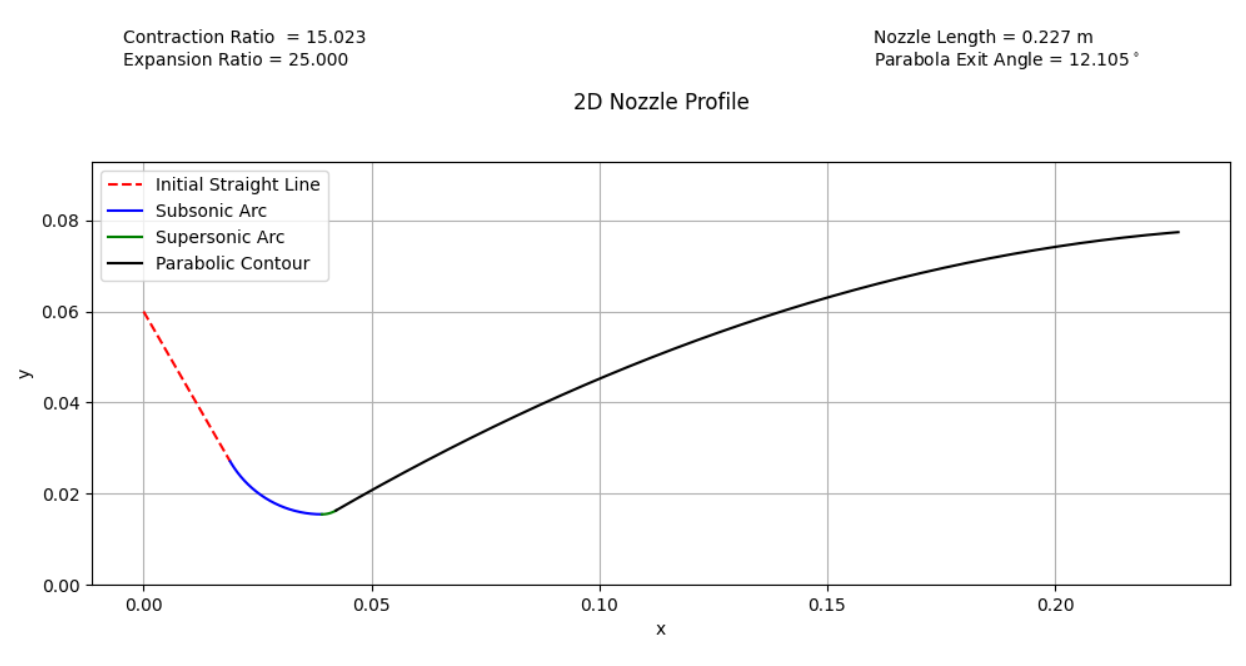
\includegraphics[width=0.85\linewidth]{Images/plot2D.png}}{\fbox{\parbox{0.78\linewidth}{\centering Missing figure file: \texttt{plot2D.png}}}}
    \caption{Example 1 of a generated two-dimensional nozzle geometry profile.}
    \label{fig:plot2D_example_2}
\end{figure}

\begin{figure}[H]
    \centering
    \IfFileExists{Images/ex3.png}{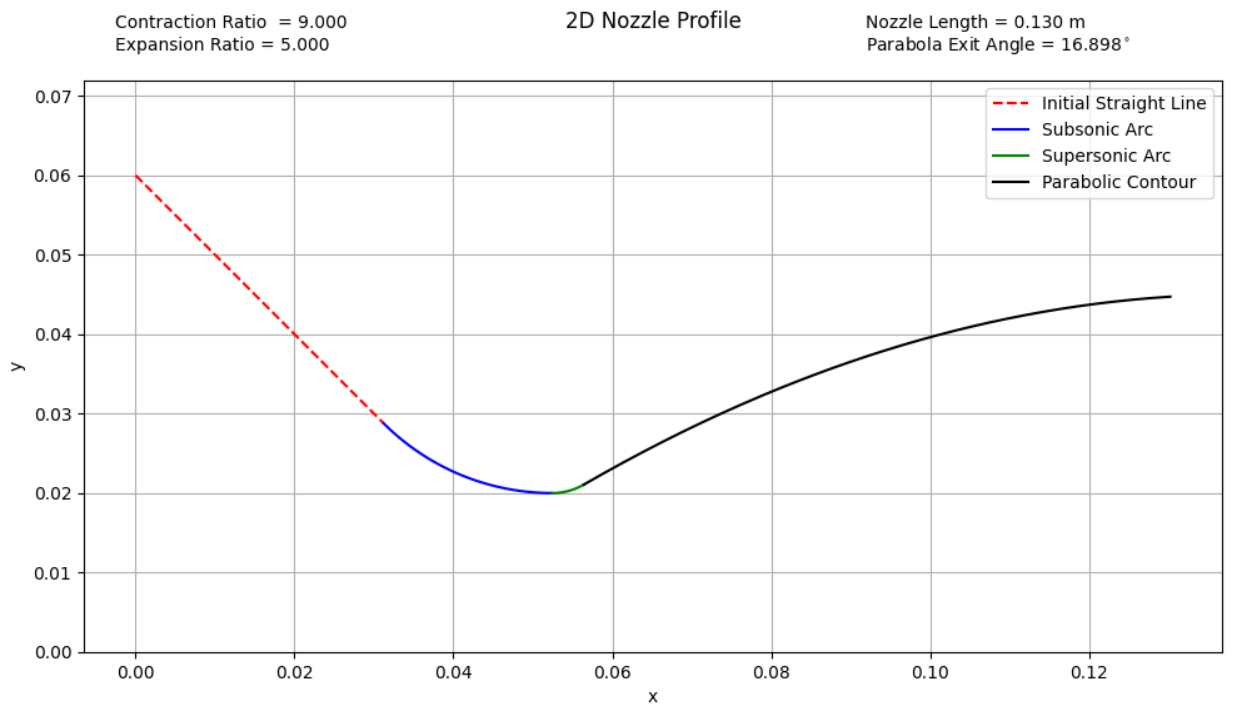
\includegraphics[width=0.85\linewidth]{Images/ex3.png}}{\fbox{\parbox{0.78\linewidth}{\centering Missing figure file: \texttt{plot2D.png}}}}
    \caption{Example 2 of a generated two-dimensional nozzle geometry profile.}
    \label{fig:plot2D}
\end{figure}

\newpage
% =========================================================
\subsection{Axisymmetric Three-Dimensional Geometry Reconstruction}
% =========================================================

\subsubsection{Surface-of-revolution definition}

Because the nozzle is axisymmetric, the three-dimensional surface is generated by revolving the two-dimensional radius function around the nozzle axis. For each axial coordinate $x_i$ and radius $r_i$, a circular ring is generated using the angular coordinate $\phi$:
\begin{align}
X_i(\phi)&=x_i,\\
Y_i(\phi)&=r_i\cos\phi,\\
Z_i(\phi)&=r_i\sin\phi,
\end{align}
with
\begin{equation}
\phi\in[0,2\pi].
\end{equation}

The complete nozzle surface is therefore
\begin{equation}
\bm{S}(x,\phi)=
\begin{bmatrix}
x\\
r(x)\cos\phi\\
r(x)\sin\phi
\end{bmatrix}.
\label{eq:surface_of_revolution}
\end{equation}

This formulation is important because it makes clear that the three-dimensional geometry is not an independent model. It is the direct revolution of the piecewise two-dimensional contour from Eq.~\eqref{eq:piecewise_nozzle}.



\subsubsection{Structured mesh matrices for visualization}

For numerical visualization, the axial and angular coordinates are assembled into matrices. If
\begin{equation}
\bm{x}=\begin{bmatrix}x_0&x_1&\cdots&x_n\end{bmatrix}^T,
\end{equation}
and
\begin{equation}
\bm{\phi}=\begin{bmatrix}\phi_0&\phi_1&\cdots&\phi_m\end{bmatrix},
\end{equation}
then the axial mesh has the structure
\begin{equation}
X=\begin{bmatrix}
x_0&x_0&\cdots&x_0\\
x_1&x_1&\cdots&x_1\\
\vdots&\vdots&\ddots&\vdots\\
x_n&x_n&\cdots&x_n
\end{bmatrix}.
\label{eq:Xmesh}
\end{equation}

The angular mesh is
\begin{equation}
\Phi=\begin{bmatrix}
\phi_0&\phi_1&\cdots&\phi_m\\
\phi_0&\phi_1&\cdots&\phi_m\\
\vdots&\vdots&\ddots&\vdots\\
\phi_0&\phi_1&\cdots&\phi_m
\end{bmatrix}.
\label{eq:Phimesh}
\end{equation}

The radial mesh is
\begin{equation}
R=\begin{bmatrix}
r_0&r_0&\cdots&r_0\\
r_1&r_1&\cdots&r_1\\
\vdots&\vdots&\ddots&\vdots\\
r_n&r_n&\cdots&r_n
\end{bmatrix}.
\label{eq:Rmesh}
\end{equation}

The Cartesian surface matrices are finally
\begin{align}
Y &= R\cos\Phi,\\
Z &= R\sin\Phi.
\end{align}

\subsubsection{Three-dimensional geometry inspection}

The three-dimensional plot is used as a quick visual validation before exporting the profile to CAD. It helps identify discontinuities, wrong radius values, exaggerated exit radius, incorrect translations, etc.

\begin{figure}[H]
    \centering
    \IfFileExists{Images/ex4.png}{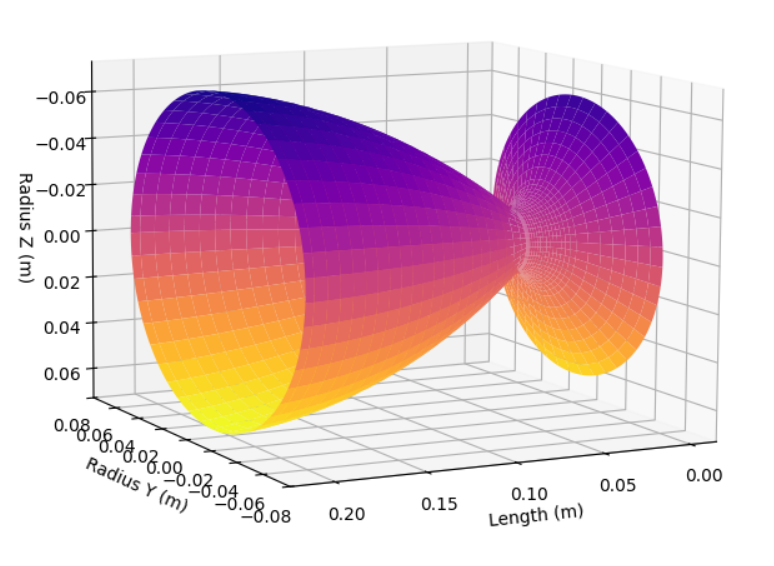
\includegraphics[width=0.84\linewidth]{Images/ex4.png}}{\fbox{\parbox{0.85\linewidth}{\centering Missing figure file: \texttt{ex4.png}}}}
    \caption{Example of three-dimensional nozzle visualization generated by surface revolution.}
    \label{fig:3D_view}
\end{figure}

\begin{figure}[H]
    \centering
    \IfFileExists{Images/ex10.png}{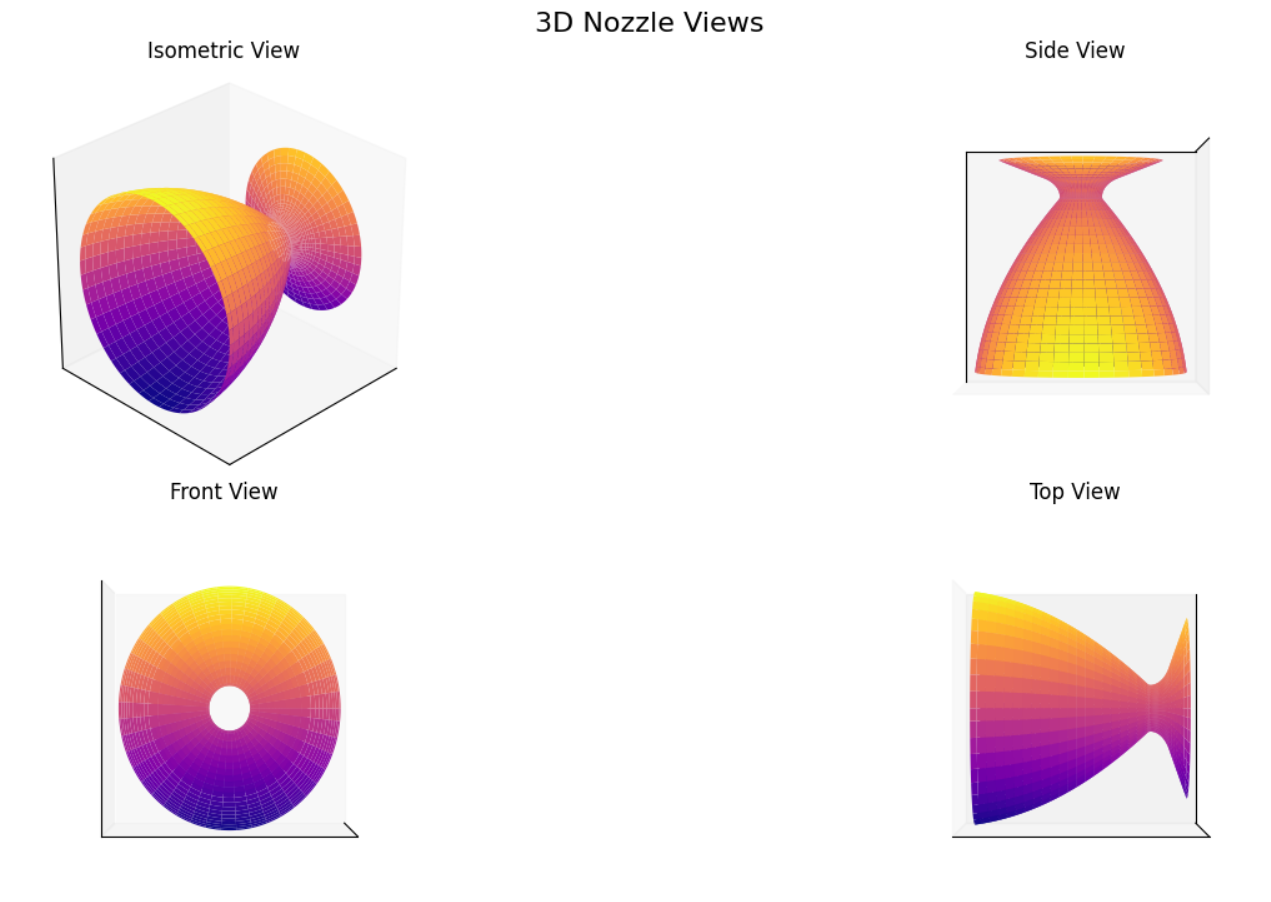
\includegraphics[width=0.88\linewidth]{Images/ex10.png}}{\fbox{\parbox{0.88\linewidth}{\centering Missing figure file: \texttt{ex10.png}}}}
    \caption{Example of multi-view visualization of the generated nozzle geometry.}
    \label{fig:3D_multiview}
\end{figure}

% =========================================================
\subsection{CAD-Oriented Geometry Export and Manufacturing Workflow}
% =========================================================

\subsubsection{CAD-compatible coordinate export}

One of the practical objectives of the simulator is to convert the numerically
generated nozzle contour into a format suitable for computer-aided design (CAD).
The exported coordinates describe the two-dimensional meridional profile of the
nozzle and can be imported into software such as Autodesk Fusion or SolidWorks.

The exported point set is written as
\begin{equation}
    \mathcal{P}
    =
    \left\{
        (x_i,r_i,0)
    \right\}_{i=0}^{N},
\end{equation}
where \(x_i\) is the axial coordinate and \(r_i\) is the corresponding wall
radius. The third coordinate is set to zero because the contour is imported as
a planar curve. Before export, the axial coordinates are translated so that the
first point of the contour is located at \(x=0\), and the coordinates are
converted from metres to millimetres.

The resulting curve represents the internal wall of the nozzle. A
three-dimensional body can subsequently be reconstructed in CAD by defining
the required wall thickness, closing the sketch and revolving the resulting
cross-section around the nozzle axis.

\subsubsection{Point reduction and sketch-conditioning strategy}

The numerical geometry uses a relatively dense point distribution to provide
smooth plots and sufficiently resolved flow, thermal and boundary-layer
profiles. Directly importing this complete point set into CAD, however, may
produce an unnecessarily complex spline. Excessive point density, particularly
near segment junctions, can lead to local oscillations, poor spline conditioning
and difficulties when applying sketch constraints.

\begin{figure}[H]
    \centering
    \begin{subfigure}{0.48\linewidth}
        \centering
        \IfFileExists{Images/ex11.png}
        {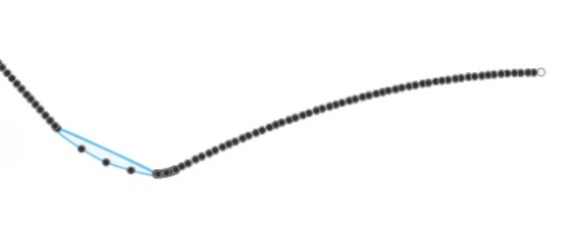
\includegraphics[width=\linewidth]{Images/ex11.png}}
        {\fbox{\parbox{0.95\linewidth}{\centering
        Missing: \texttt{ex11.png}}}}
        \caption{Spline irregularity caused by an excessively dense point set.}
    \end{subfigure}
    \hfill
    \begin{subfigure}{0.48\linewidth}
        \centering
        \IfFileExists{Images/ex12.png}
        {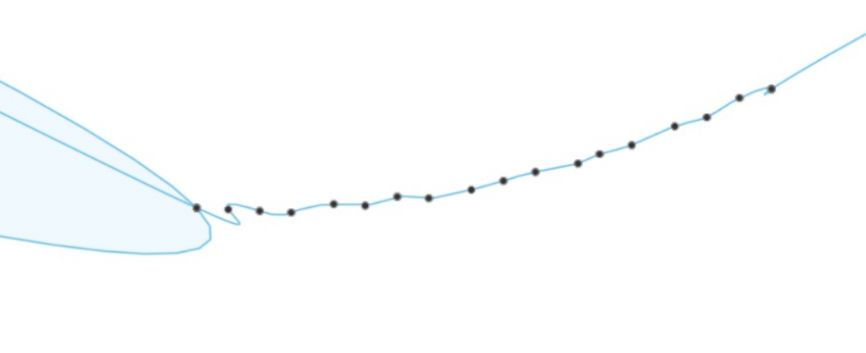
\includegraphics[width=\linewidth]{Images/ex12.png}}
        {\fbox{\parbox{0.95\linewidth}{\centering
        Missing: \texttt{ex12.png}}}}
        \caption{Detailed view of the spline near the throat transition.}
    \end{subfigure}
    \caption{CAD sketch irregularities associated with an unsuitable point
    distribution.}
    \label{fig:cad_irregularity}
\end{figure}


The initial CAD-export implementation therefore included a two-stage
point-conditioning procedure. First, a target of approximately 100 points was
distributed proportionally among the four geometric regions:
\begin{enumerate}
    \item the straight convergent section;
    \item the subsonic throat arc;
    \item the supersonic throat arc;
    \item the parabolic bell contour.
\end{enumerate}
A minimum of two points was retained in each region so that no geometric segment
was omitted. Within each segment, points were selected at approximately uniform
index intervals.

A second sequential filter was then applied to remove clustered points. A
candidate point was retained only when its distance from the previously accepted
point satisfied
\begin{equation}
    d_i
    =
    \sqrt{
        (x_i-x_k)^2+(r_i-r_k)^2
    }
    \geq d_{\min},
\end{equation}
where \(k\) denotes the last accepted point and \(d_{\min}\) is the prescribed
minimum spacing. A value of approximately
\(d_{\min}=1\,\mathrm{mm}\) was used during the CAD-conditioning tests. The
first and final contour points, together with the points defining the main
geometric transitions, should be preserved explicitly to maintain the chamber
inlet, throat and nozzle-exit dimensions.

The current modular implementation exports the complete set of unique geometry
points to \texttt{geometry.csv}. The reduction procedure described above
corresponds to the CAD-conditioning stage developed in the initial version and
can be applied as an additional preprocessing step when a lighter CAD spline is
required.


\subsubsection{CAD reconstruction workflow}

The complete geometry-reconstruction workflow is summarized as follows:
\begin{enumerate}
    \item generate the two-dimensional contour using the geometric model;
    \item translate the axial coordinates so that the contour begins at \(x=0\);
    \item remove duplicate points at the junctions between geometric segments;
    \item reduce and filter the point set when CAD conditioning is required;
    \item convert the coordinates from metres to millimetres;
    \item export the coordinates as a three-column point file;
    \item import the point file into the CAD environment;
    \item create a spline through the imported points;
    \item define the wall thickness by offsetting the internal contour;
    \item close the cross-section and revolve it around the nozzle axis.
\end{enumerate}

%\begin{figure}[H]
%    \centering
%    \IfFileExists{Images/ex13.png}
%    {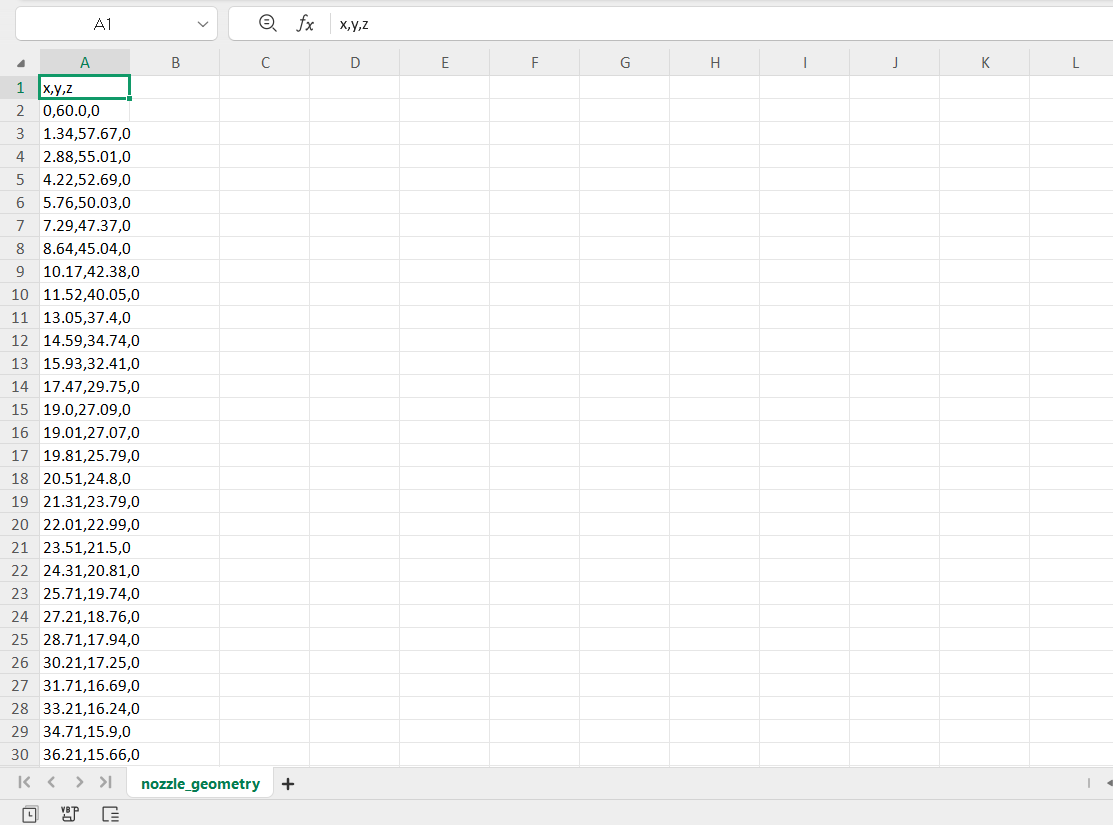
\includegraphics[width=0.85\linewidth]{Images/ex13.png}}
%    {\fbox{\parbox{0.85\linewidth}{\centering
 %   Missing figure file: \texttt{ex13.png}}}}
  %  \caption{Example of the exported nozzle-coordinate file opened in tabular
  %  form.}
  %  \label{fig:csv_output}
%\end{figure}

\begin{figure}[H]
    \centering
    \IfFileExists{Images/ex14.png}
    {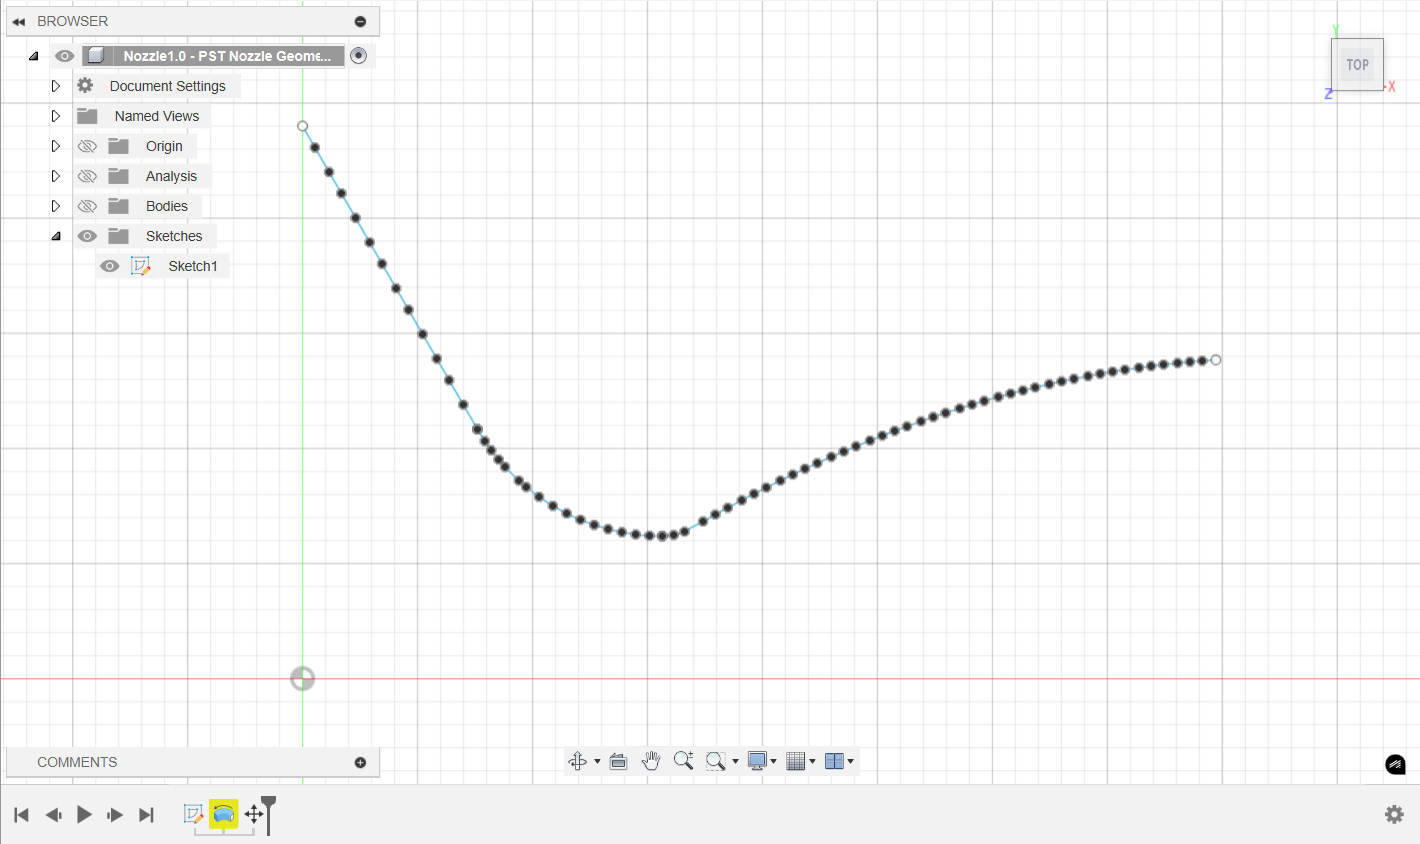
\includegraphics[width=0.78\linewidth]{Images/ex14.png}}
    {\fbox{\parbox{0.78\linewidth}{\centering
    Missing figure file: \texttt{ex14.png}}}}
    \caption{Nozzle contour reconstructed in CAD using the conditioned point
    distribution.}
    \label{fig:cad_sketch}
\end{figure}

\begin{figure}[H]
    \centering
    \begin{subfigure}{0.48\linewidth}
        \centering
        \IfFileExists{Images/ex16.png}
        {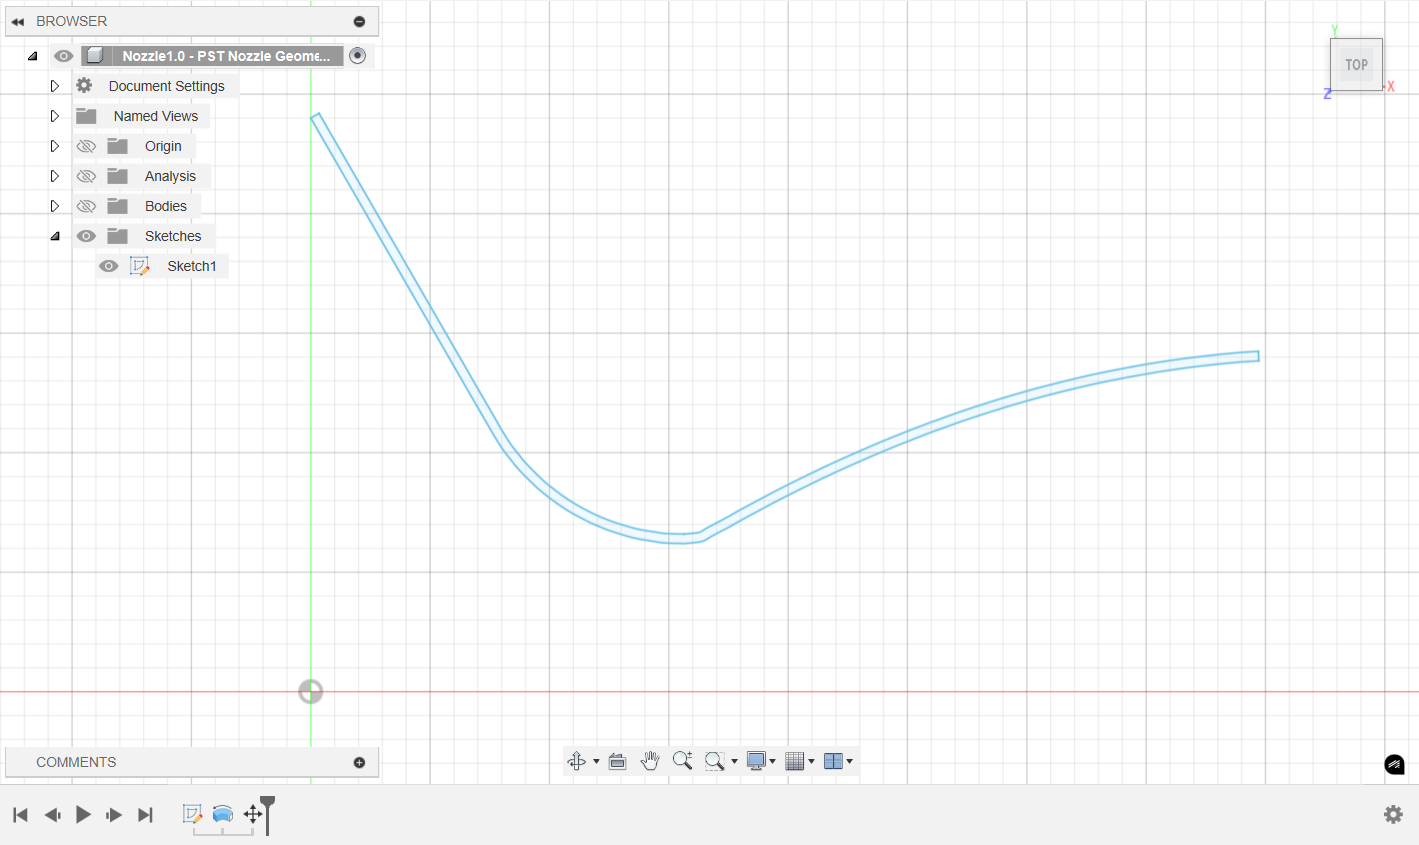
\includegraphics[width=\linewidth]{Images/ex16.png}}
        {\fbox{\parbox{0.95\linewidth}{\centering
        Missing: \texttt{ex16.png}}}}
        \caption{Definition of the nozzle wall thickness.}
    \end{subfigure}
    \hfill
    \begin{subfigure}{0.48\linewidth}
        \centering
        \IfFileExists{Images/ex17.png}
        {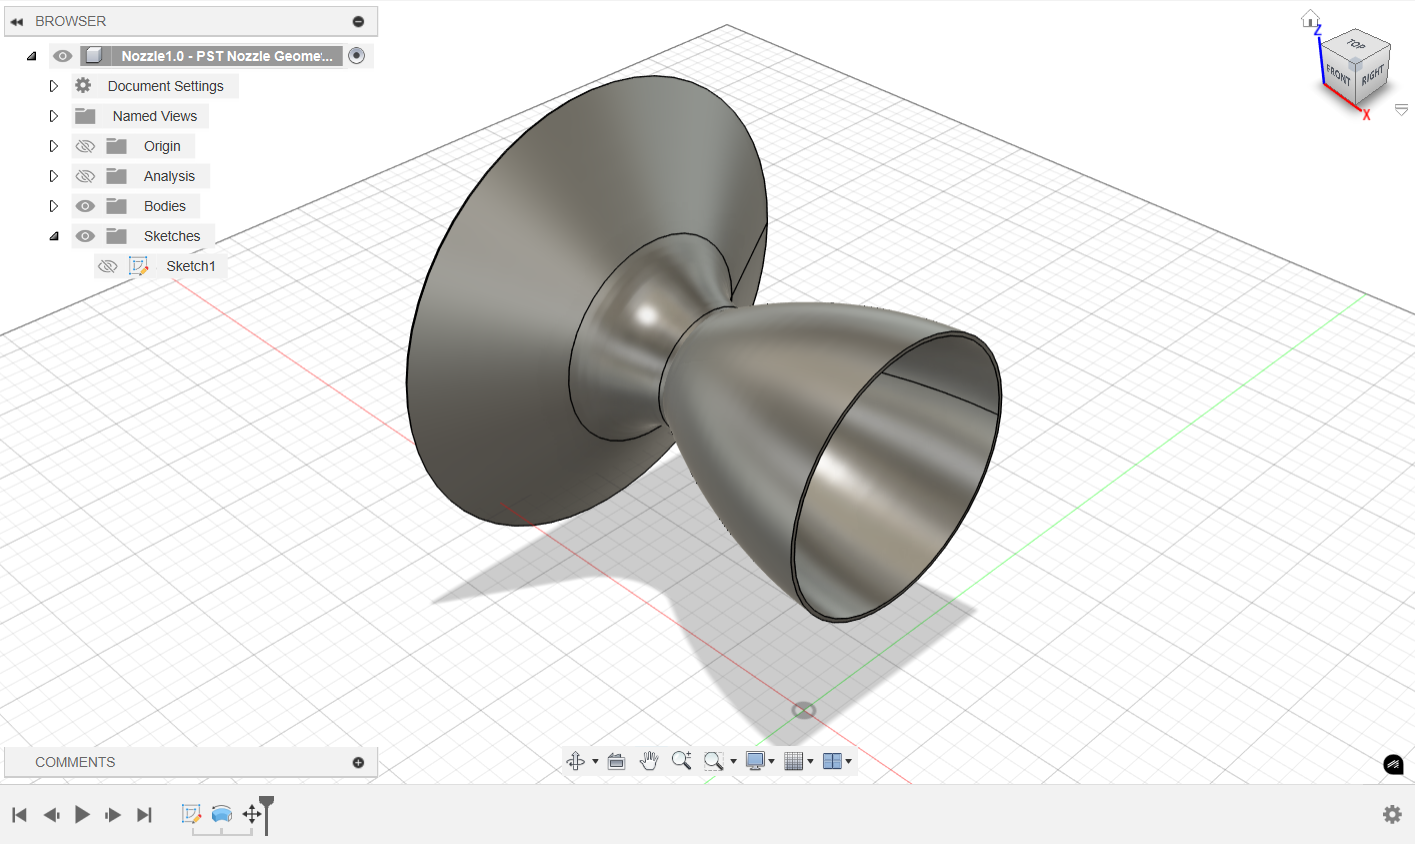
\includegraphics[width=\linewidth]{Images/ex17.png}}
        {\fbox{\parbox{0.95\linewidth}{\centering
        Missing: \texttt{ex17.png}}}}
        \caption{Final axisymmetric nozzle body after revolution.}
    \end{subfigure}
    \caption{CAD operations used to convert the exported meridional contour
    into a manufacturable three-dimensional body.}
    \label{fig:cad_final}
\end{figure}
